% !TEX root = cha-application.tex
\documentclass[../../main.tex]{subfiles}

\begin{document}

\section{Evaluation of Backtracking Strategies}
\label{sec:backtracking_evaluation}

In this experiment, we compare five backtracking strategies for handling contradictions during WFC path generation. We used the complete class hierarchy of the Pharo 13 \texttt{HashedCollection} class (\figref{fig:hashedCollection_hierarchy}).

\begin{figure}[ht]
    \centering
    \includegraphics[width=0.7\linewidth]{figures/application/hashedCollection_hierarchy.pdf}
    \caption{\texttt{HashedCollection} full hierarchy.}
    \label{fig:hashedCollection_hierarchy}
\end{figure}

For each of the 5 strategies, we ran 24 instances for 4 hours. All other configuration parameters were kept the same. In total, 120 instances were executed, and the initial grid had an average size of $31.12 \times 31.12$ cells.

During each generation, the solver allowed up to 5 backtracks on the same grid. If no solution was found, it discarded the current class placement and started again with the same grid size.

The five strategies were:

\begin{itemize}
    \item \textbf{Fixed Number of Steps:} Goes back a fixed number of collapse steps. We used 50 steps.
    \item \textbf{Percentage of Steps:} Goes back by a fixed percentage of the collapse steps. We used 20\%.
    \item \textbf{Many Possible Tiles:} Goes back to a checkpoint saved before a cell with many possible tiles was collapsed. The minimum number of tiles was 7.
    \item \textbf{Similar Tile Weights:} Goes back to a checkpoint saved before a cell with similar tile weights was collapsed. This was triggered when at least 30\% of the candidate tiles had a maximum weight difference of 20\%.
    \item \textbf{Restart:} Discards the current solution and starts the path generation from the beginning.
\end{itemize}

\subsection{Experimental Results and Analysis}
\label{subsec:backtracking_results}

The results are shown in \figref{fig:backtracking_results}. Out of 24 instances, the strategies solved:

\begin{itemize}
    \item \textbf{Fixed Number of Steps:} 17 instances (70.8\%).
    \item \textbf{Percentage of Steps:} 19 instances (79.2\%).
    \item \textbf{Many Possible Tiles:} 16 instances (66.7\%).
    \item \textbf{Similar Tile Weights:} 20 instances (83.3\%).
    \item \textbf{Restart:} 21 instances (87.5\%).
\end{itemize}

The boxplots in \figref{fig:backtracking_boxplot} show the execution times, while the cactus plot in \figref{fig:backtracking_cactus} shows how many instances were solved over time.

The results are similar for the five strategies, but the \textbf{Restart} strategy solved the most instances and generally found solutions faster.

One possible reason is the small size of the tested system. For a class hierarchy such as \texttt{HashedCollection}, a contradiction can be caused by an early class placement that makes the rest of the grid difficult to solve. In this case, going back step by step may spend time trying to fix a layout that is already difficult to solve.

With \textbf{Restart}, the solver can discard this layout and try a new class placement immediately. For this relatively small system, starting again has a low cost.

For larger and more complex systems, this may change~\citebibliography{Karth2022a}. In such cases, restarting from the beginning can waste more work, while backtracking strategies that keep part of the current solution may become more useful.

\begin{figure}[ht]
    \centering
    \begin{subfigure}[b]{0.65\textwidth}
        \centering
        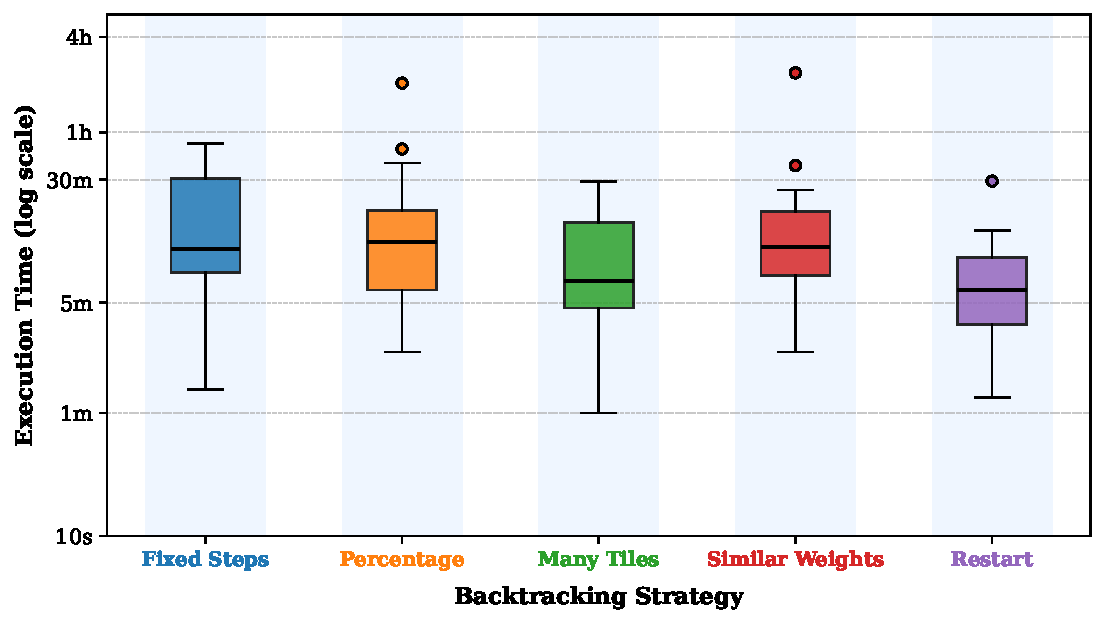
\includegraphics[width=\textwidth]{figures/application/backtracking_strategies_boxplot}
        \caption{Execution times.}
        \label{fig:backtracking_boxplot}
    \end{subfigure}
    \hfill
    \begin{subfigure}[b]{0.65\textwidth}
        \centering
        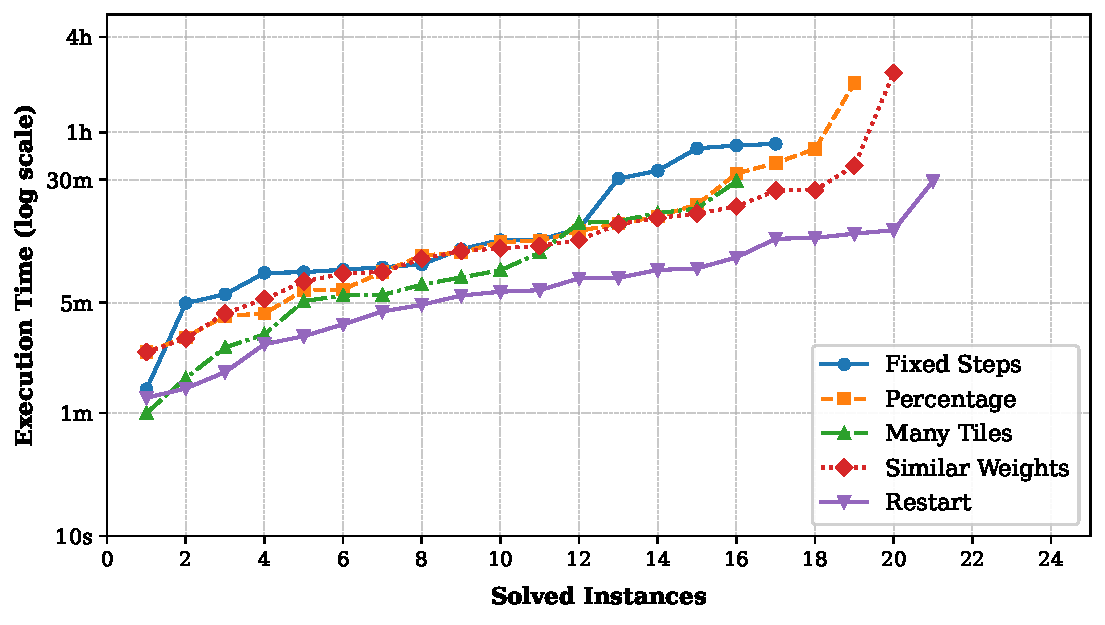
\includegraphics[width=\textwidth]{figures/application/backtracking_strategies_cactus}
        \caption{Solved instances over time.}
        \label{fig:backtracking_cactus}
    \end{subfigure}
    \caption{Results for the five backtracking strategies.}
    \label{fig:backtracking_results}
\end{figure}

\end{document}